\documentclass{article}
\usepackage{iftex}
\ifPDFTeX
  \usepackage[utf8]{inputenc}
  \usepackage[T1]{fontenc}
  \usepackage{lmodern}
  \usepackage{textcomp}
\else
  \usepackage{fontspec}
\fi
\usepackage{amssymb}
\usepackage{booktabs}
\usepackage{graphicx}
\usepackage{hyperref}
\usepackage{xcolor}
\usepackage{newunicodechar}
\newunicodechar{α}{\ensuremath{\alpha}}
\newunicodechar{β}{\ensuremath{\beta}}
\newunicodechar{γ}{\ensuremath{\gamma}}
\newunicodechar{δ}{\ensuremath{\delta}}
\newunicodechar{ε}{\ensuremath{\varepsilon}}
\newunicodechar{ζ}{\ensuremath{\zeta}}
\newunicodechar{η}{\ensuremath{\eta}}
\newunicodechar{θ}{\ensuremath{\theta}}
\newunicodechar{ι}{\ensuremath{\iota}}
\newunicodechar{κ}{\ensuremath{\kappa}}
\newunicodechar{λ}{\ensuremath{\lambda}}
\newunicodechar{μ}{\ensuremath{\mu}}
\newunicodechar{ν}{\ensuremath{\nu}}
\newunicodechar{ξ}{\ensuremath{\xi}}
\newunicodechar{π}{\ensuremath{\pi}}
\newunicodechar{ρ}{\ensuremath{\rho}}
\newunicodechar{ς}{\ensuremath{\varsigma}}
\newunicodechar{σ}{\ensuremath{\sigma}}
\newunicodechar{τ}{\ensuremath{\tau}}
\newunicodechar{υ}{\ensuremath{\upsilon}}
\newunicodechar{φ}{\ensuremath{\varphi}}
\newunicodechar{χ}{\ensuremath{\chi}}
\newunicodechar{ψ}{\ensuremath{\psi}}
\newunicodechar{ω}{\ensuremath{\omega}}
\newunicodechar{Γ}{\ensuremath{\Gamma}}
\newunicodechar{Δ}{\ensuremath{\Delta}}
\newunicodechar{Θ}{\ensuremath{\Theta}}
\newunicodechar{Λ}{\ensuremath{\Lambda}}
\newunicodechar{Ξ}{\ensuremath{\Xi}}
\newunicodechar{Π}{\ensuremath{\Pi}}
\newunicodechar{Σ}{\ensuremath{\Sigma}}
\newunicodechar{Υ}{\ensuremath{\Upsilon}}
\newunicodechar{Φ}{\ensuremath{\Phi}}
\newunicodechar{Ψ}{\ensuremath{\Psi}}
\newunicodechar{Ω}{\ensuremath{\Omega}}
\newunicodechar{≤}{\ensuremath{\leq}}
\newunicodechar{≥}{\ensuremath{\geq}}
\newunicodechar{≈}{\ensuremath{\approx}}
\newunicodechar{≠}{\ensuremath{\neq}}
\newunicodechar{≡}{\ensuremath{\equiv}}
\newunicodechar{∝}{\ensuremath{\propto}}
\newunicodechar{∈}{\ensuremath{\in}}
\newunicodechar{∉}{\ensuremath{\notin}}
\newunicodechar{⊂}{\ensuremath{\subset}}
\newunicodechar{⊃}{\ensuremath{\supset}}
\newunicodechar{⊆}{\ensuremath{\subseteq}}
\newunicodechar{⊇}{\ensuremath{\supseteq}}
\newunicodechar{∪}{\ensuremath{\cup}}
\newunicodechar{∩}{\ensuremath{\cap}}
\newunicodechar{∅}{\ensuremath{\emptyset}}
\newunicodechar{∀}{\ensuremath{\forall}}
\newunicodechar{∃}{\ensuremath{\exists}}
\newunicodechar{√}{\ensuremath{\surd}}
\newunicodechar{∑}{\ensuremath{\sum}}
\newunicodechar{∏}{\ensuremath{\prod}}
\newunicodechar{∫}{\ensuremath{\int}}
\newunicodechar{∞}{\ensuremath{\infty}}
\newunicodechar{∂}{\ensuremath{\partial}}
\newunicodechar{∇}{\ensuremath{\nabla}}
\newunicodechar{→}{\ensuremath{\rightarrow}}
\newunicodechar{←}{\ensuremath{\leftarrow}}
\newunicodechar{↔}{\ensuremath{\leftrightarrow}}
\newunicodechar{⇒}{\ensuremath{\Rightarrow}}
\newunicodechar{⇐}{\ensuremath{\Leftarrow}}
\newunicodechar{⇔}{\ensuremath{\Leftrightarrow}}
\newunicodechar{−}{\ensuremath{-}}
\newunicodechar{±}{\ensuremath{\pm}}
\newunicodechar{∓}{\ensuremath{\mp}}
\newunicodechar{×}{\ensuremath{\times}}
\newunicodechar{÷}{\ensuremath{\div}}
\newunicodechar{⋅}{\ensuremath{\cdot}}
\newunicodechar{∘}{\ensuremath{\circ}}
\newunicodechar{⊗}{\ensuremath{\otimes}}
\newunicodechar{⊕}{\ensuremath{\oplus}}
\newunicodechar{′}{\ensuremath{\prime}}
\newunicodechar{ℝ}{\ensuremath{\mathbb{R}}}
\newunicodechar{ℕ}{\ensuremath{\mathbb{N}}}
\newunicodechar{ℤ}{\ensuremath{\mathbb{Z}}}
\newunicodechar{ℚ}{\ensuremath{\mathbb{Q}}}
\newunicodechar{ℂ}{\ensuremath{\mathbb{C}}}
\newunicodechar{—}{\textemdash{}}
\newunicodechar{–}{\textendash{}}
\newunicodechar{…}{\ldots{}}
\newunicodechar{§}{\S{}}
\newunicodechar{¶}{\P{}}
\newunicodechar{·}{\textperiodcentered{}}
\newunicodechar{°}{\textdegree{}}
\newunicodechar{²}{\textsuperscript{2}}
\newunicodechar{³}{\textsuperscript{3}}
\newunicodechar{¹}{\textsuperscript{1}}
\newunicodechar{⁰}{\textsuperscript{0}}
\newunicodechar{⁴}{\textsuperscript{4}}
\newunicodechar{⁵}{\textsuperscript{5}}
\newunicodechar{⁶}{\textsuperscript{6}}
\newunicodechar{⁷}{\textsuperscript{7}}
\newunicodechar{⁸}{\textsuperscript{8}}
\newunicodechar{⁹}{\textsuperscript{9}}
\newunicodechar{‘}{\textquoteleft{}}
\newunicodechar{’}{\textquoteright{}}
\newunicodechar{“}{\textquotedblleft{}}
\newunicodechar{”}{\textquotedblright{}}
\definecolor{validated}{HTML}{047857}
\definecolor{refuted}{HTML}{B91C1C}
\definecolor{inconclusive}{HTML}{9A3412}
\title{Empirical Proof Record: VALIDATED}
\date{2026-05-24T17:57:18.252037+00:00}
\begin{document}
\maketitle
\section*{Empirical Proof Record --- \textcolor{validated}{\textbf{VALIDATED}}}
\textbf{Proof ID:} \texttt{c1c889feafde5139a20f0ecf7ca35f0f\dots}\\
\textbf{Created:} 2026-05-24T17:57:18.252037+00:00
\subsection*{1. Claim}
\begin{quote}On the live substrate, growing the geoid dimension mid-session via \_refit\_geoid\_dimension (re-fit on the substrate's own lived cloud, grow-only, N=IPR) keeps the cognitive cycle coherent — post-grow mean Φ >= 0.5 — where a naive dimension swap collapses it (Φ=0, stale Ymir + F2 drift). N grows with accumulated experience.\end{quote}
\begin{itemize}
\item \textbf{Operationalisation:} Learned-N Takwin at N=16 → warm-up cycles on real BGE words → \_refit\_geoid\_dimension() (N=round IPR of the lived \_geoid\_map) → post-grow cycles; observed = post-grow mean Φ, gated on grew=True. (Measured in the Kimera venv; signed from the cache.)
\item \textbf{Threshold:} \texttt{post\_grow\_mean\_phi >= 0.5 phi}
\item \textbf{H0:} H0: post-grow mean Φ < 0.5 or N did not grow — a live mid-session grow degrades cognition
\item \textbf{H1:} H1: post-grow mean Φ >= 0.50 and N grew — runtime dynamic-N is viable
\end{itemize}
\subsection*{2. Verdict}
\textcolor{validated}{\textbf{VALIDATED}} --- observed \texttt{0.638}\\
live mid-session grow N 16→71 (IPR 71.0, 152 geoids re-projected, grew=True); post-grow mean Φ 0.638 over 5 cycles (pre-grow 0.652); naive-swap baseline Φ=0 (stale Ymir + F2 drift; journals 077/079) — the method's resets keep the cycle coherent
\begin{figure}[h!]\centering
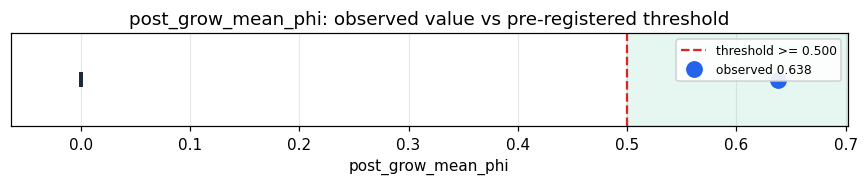
\includegraphics[width=0.8\linewidth]{assets/ci_post_grow_mean_phi}
\caption{post\_grow\_mean\_phi -- observed value with Wilson 95\% CI.}
\end{figure}
\subsection*{3. Evidence}
\begin{tabular}{llrrl}\toprule
\textbf{Pillar} & \textbf{Statistic} & \textbf{Value} & \textbf{95\% CI} & \textbf{Library} \\\midrule
\texttt{runtime\_dynamic\_n\_coherent} & \texttt{post\_grow\_mean\_phi} & \texttt{0.638} & (0.0000, 0.0000) & numpy 2.4.4 \\
\bottomrule\end{tabular}
\subsection*{4. Pre-registration}
\begin{itemize}
\item Registered at: \texttt{2026-05-24T17:57:17.824255+00:00}
\item Config hash: \texttt{c84c34eae94682a0f9c02e4bae6eaea4\dots}
\item Data hash: \texttt{8193bfba90344687c19a747691d10b4b\dots}
\end{itemize}
\subsection*{5. Signature}
\texttt{d95bd0ec980ebb2b09d1537a768be29ce565ccb62f0ef370754f5876e061383b}\\

\end{document}
